\documentclass{article}
\usepackage{listing}
\usepackage{csp}
\usepackage{cspm}
\usepackage{helper}
\usepackage{tikz}
\usetikzlibrary{arrows.meta}
\usetikzlibrary{positioning}
\usetikzlibrary{decorations.text}

\begin{document}
\section{Linearization}
Proving a concurrent datatype's correctness is usually more complicated than proving for a single-threaded data structure. In addition to the state explosion when more and more processes are involved, scheduling is one particular reason that proving is difficult. For example, two processes are enqueuing their data to a concurrent queue. The process calling earlier may be descheduled and interact with the queue after the other process.

The linearizability test from [TODO:reference] is one way to prove that a sequence of process interactions is correct using only trivially measurable information - pairs of calling and returning time of every function call made by every process.   From the history of function calls, The linearizability test tries to find a synchronization point for each call, where the call appears to make an effect. In addition, the series of synchronization points should satisfy the specification of the concurrent datatype.

In order to show that a system using a concurrent datatype is correct, the linearizability test works by running the system many times and checking the traces. In this essay, we use CSP models and the linearizer framework to prove the correctness of a concurrent datatype.

CSP is ... Trace is ... Trace refinement is ... FDR is ...

In the CSP model, the history of all function call is represented using related events. \CSPM{Call.t.op.p} represents a process calls function \CSPM{op} with parameter \CSPM{p}. \CSPM{Return.t.op.ans} represents a process returns from calling \CSPM{op} with return value \CSPM{ans}.

In CSP, trace refinement is a valuable tool to analyze the history of function calls described in the linearizability test. If the testing system, which produces possible function calls and function returns in CSP, refines a CSP specification of the system, then the testing system cannot do anything incorrect and thus must be correct. One way to construct the specification is to use the linearizer framework.

The linearizer has two core components - the linearizer process and the specification process for the \CSPM{Sync} event. The linearizer process generates endless pairs of \CSPM{Call} and \CSPM{Return} events with its synchronization point for a specific process. When all linearizer processes, together with the specification process for \CSPM{Sync}, run in parallel, the combined process produces all possible histories in CSP. Figure \ref{intro.linearizer.combine} shows how to create the combined processes in FDR. In Section ... we shall see more concrete instances of the linearizer framework.
\begin{cspinline}{intro.linearizer.combine}{Creation of the specification from the linearizers}
(( || me: All @ [LinEvents(All,me)]  Lin(All,me)) [|{|Sync|}|] Spec) \ {|Sync|}
\end{cspinline}
\section{Common Objects}
\subsection{Shared Variable}
The usage of shared variables is common in concurrent datatypes. For example, some concurrent datatypes may temporarily store the identity of a waiting process. However, CSP is more like a functional programming language and does not support mutable variables. 

A recursive process in CSP can capture the behaviour of a shared variable. The recursive process holds the value of the variable in its parameter. At any time, the variable process is willing to answer a query for the variable value in channel \CSPM{getValue}. Alternatively, the process can receive an update on the variable value in channel \CSPM{getValue}, after which the function recurses with the new variable value.

Because it is natural for a concurrent datatype to use multiple shared variables, the global variable is implemented as a CSP module, as shown in Figure \ref{globalvar.csp}. The module requires two parameters. \CSPM{TypeValue} is the set of possible values for the variable, and \CSPM{initialValue} is the value before any process modifies the variable. An uninitialized variable module is also available in the same figure \ref{globalvar.csp}, with the only difference that the variable non-deterministically chooses an initial value from \CSPM{TypeValue} at start time. \CSPM{runWith} is a convenient helper function to run a given process \CSPM{P} with the \CSPM{Var} process. If the parameter \CSPM{hide} is true, \CSPM{runWith} function hides all events introduced by the shared variable. In later chapters, we will see how the \CSPM{runWith} function helps reduce the code complexity of the synchronization object implementation.

\begin{cspinline}{globalvar.csp}{CSP implementation of global variable process module}
module ModuleVariable(TypeValue, initialValue)
  Var(value) = getValue!value -> Var(value)
             [] setValue?value -> Var(value)
  chanset = {|getValue, setValue|}
exports
  //(Bool, Proc) -> Proc
  runWith(hide,P) = if hide then (Var(initialValue) [|chanset|] P) \ chanset
                            else  Var(initialValue) [|chanset|] P
  channel getValue, setValue: TypeValue
endmodule

module ModuleUninitVariable(TypeValue)
  Var(value) = getValue!value -> Var(value)
            [] setValue?value -> Var(value)
  chanset = {|getValue, setValue|}
exports
  runWith(hide,P) = 
    if hide then ((|~| x:TypeValue @ Var(x)) [| chanset |] P) \ chanset
    else (|~| x:TypeValue @ Var(x)) [| chanset |] P
  channel getValue, setValue: TypeValue
endmodule
\end{cspinline}

Figure \ref{globalvar.csp.example} is an example of two processes using a shared variable. The first line in the example creates a shared variable \CSPM{VarA} with value ranging from $0$ to $2$ and initialized with $0$. Process \CSPM{P} increments \CSPM{VarA} modulo $3$ forever and process \CSPM{Q} reads \CSPM{VarA} forever. Process \CSPM{P} interleaves with process \CSPM{Q}, and the combined process is further synchronized with the variable \CSPM{VarA} process. In the resulting process \CSPM{System}, changes to \CSPM{VarA} made by process \CSPM{P} is visible to process \CSPM{Q}.

\begin{cspinline}{globalvar.csp.example}{CSP Example of a process using a shared variable}
instance VarA = ModuleVariable({0..2},0)
P = VarA::getValue?a -> VarA::setValue!((a+1)%3) -> P
Q = VarA::getValue?a -> Q
System = VarA::runWith(false,P|||Q)
\end{cspinline}


\subsection{Semaphore}
Semaphore is a simple but powerful concurrent primitive. The essay shall describe and use a simplified binary semaphore from [TODO: Reference], which removes interrupts and timeout operations. 

A binary semaphore can either be raised or unraised. A \CSPM{down} function call, usually by a process that previously acquired the semaphore, raises the semaphore regardless of the semaphore state. If a process calls the \CSPM{up} method when the semaphore is raised, the semaphore becomes unraised. However, if the semaphore is unraised, the process waits until another process calls \CSPM{down} and proceeds to put down the semaphore. Depending on the initial state of the semaphore, a binary semaphore can be further classified as a mutex semaphore or a signalling semaphore.

Modelling a semaphore is simple in CSP. A process may call \CSPM{up} function or \CSPM{down} function via channel \CSPM{upChan} or channel \CSPM{downChan} respectively. The semaphore is modelled by a process implemented by two mutually recursive functions \CSPM{Semaphore(True)} and \CSPM{Semaphore(False)}. The semaphore process representing an unraised state accepts a \CSPM{upChan} event by any process and proceeds to the raised process. The semaphore process representing a raised state can either accept a \CSPM{upChan} event and recurse to the raised process, or accept a \CSPM{downChan} event and proceed to the unraised process.

\begin{cspinline}{semaphore.csp}{Implementation of a binary semaphore in CSP}
module ModuleSemaphore(TypeThreadID, initialState)
  --Raised
  Semaphore(True) = downChan?id -> Semaphore(False)
                   [] upChan?id -> Semaphore(True)
  --Unraised
  Semaphore(False)= upChan?id   -> Semaphore(True)
  
  chanset = {|upChan, downChan|}
exports
  --runWith::(Bool,Proc) -> Proc
  runWith(hide,P) = (Mutex [| chanset |] P) \ 
                     (if hide then chanset else {})
  channel upChan, downChan: TypeThreadID
endmodule
\end{cspinline}

\subsection{Monitor}
A Monitor is another powerful concurrent primitive. This essay will also use a simplified monitor from [TODO:reference].

\begin{scalainline}{monitor.scala.example}{Description}
class MenWomen {
  private var a = 0;
  def op1():Unit = synchronized{
    a+=1;
  }
}
\end{scalainline}

Usually, code (protected by the monitor) is wrapped inside a synchronized block, as shown in Figure \ref{monitor.scala.example}. But before the process runs code inside the synchronized block, the process needs to check if others have obtained the monitor lock. Also, an exiting process needs to release the monitor lock so that other processes can continue. In Figure \ref{monitor.states}, edge 1 represents a process entering the synchronized block, and edge 6 describes the transition of a process exiting the synchronized block. Inside the synchronized block, the process may call \CSPM{notify}, \CSPM{notifyAll}, \CSPM{wait} function. A running process calling \CSPM{wait} blocks execution and waits to be notified. When a running process notifies a waiting process, the waiting process becomes runnable and waits to obtain the monitor lock. Note that the waiting process can only continue execution after the current process exits its synchronized block, unlike that a process waiting to acquire the semaphore can immediately continue after another process raises the semaphore. All above transitions are represented by edge 2,3,4,5 in diagram \ref{monitor.states} respectively. 

\begin{figure}
  \centering
  \resizebox{\linewidth}{!}{
  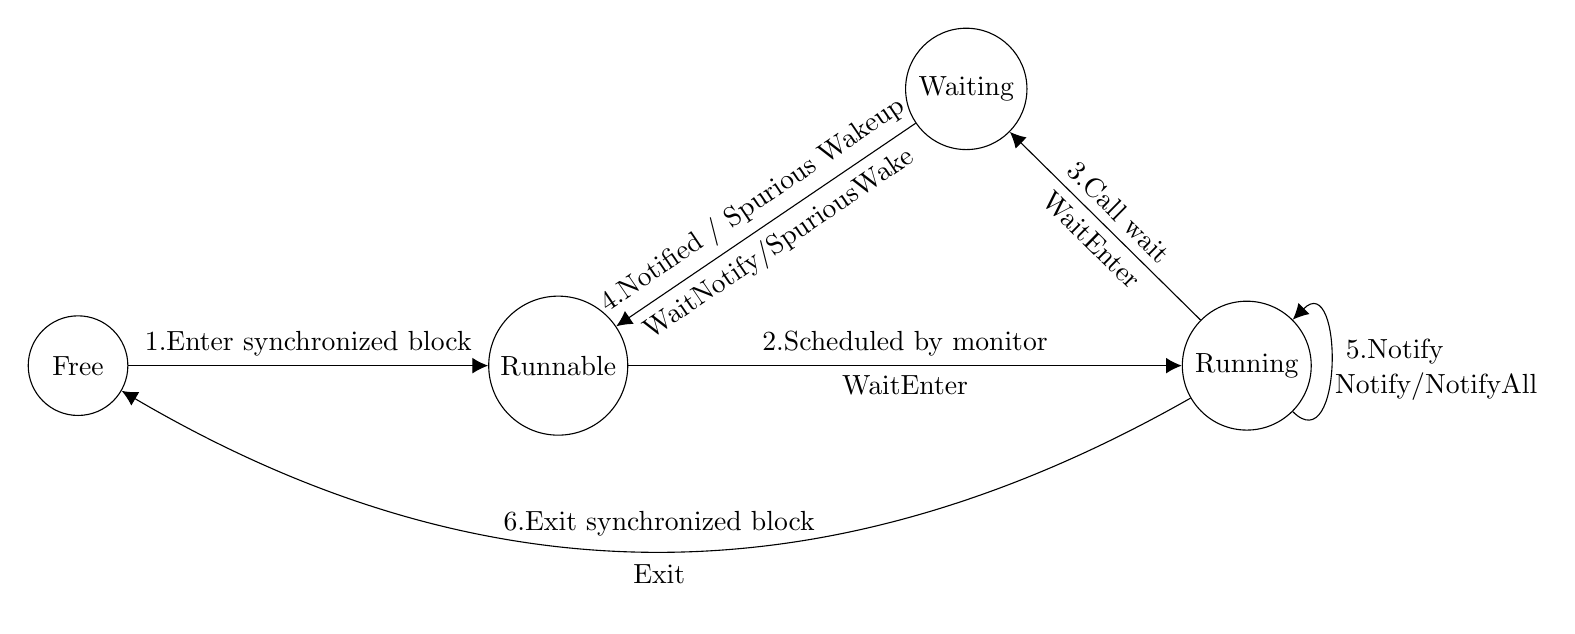
\begin{tikzpicture}[] 
      \tikzstyle{node}=[
          draw,
          circle,
          minimum size=3.6em
      ]
      \tikzstyle{edge}=[
          -{Latex[length=2mm, width=2mm]}
      ]
      \tikzset{near start abs/.style={xshift=1cm}}
      \node[node] (1) {Free}; 
      \node[node] [right=13em of 1] (2) {Runnable}; 
      \node[node] [right=20em of 2] (3) {Running};
      \node[node] [right=10em of 2, yshift=10em] (4) {Waiting};
      
      \draw[edge] (1) -- node[midway, above, sloped]{1.Enter synchronized block} node[midway, below, sloped] {} (2) ;
      \draw[edge] (2) -- node[midway, above, sloped]{2.Scheduled by monitor} node[midway, below, sloped] {\CSPM{WaitEnter}} (3) ;
      \draw[edge] (3) -- node[midway, above, sloped]{3.Call \CSPM{wait}} node[midway, below, sloped] {\CSPM{WaitEnter}} (4);
      \draw[edge] (4) -- node[midway, above, sloped]{4.Notified / Spurious Wakeup} node[midway, below, sloped] {\CSPM{WaitNotify}/\CSPM{SpuriousWake}} (2) ;
  
      \draw[edge,bend right=330] (3) to (1);
      \node[] [xshift=21em,yshift=-5.7em] (10) {6.Exit synchronized block};
      \node[] [below of=10, yshift=1em]{\CSPM{Exit}};
  
      \draw[edge] (3) to [out=315,in=45,looseness=2] (3);
      \node[] [right of=3, xshift=2.5em,yshift=0.5em] (11) {5.Notify};
      \node[] [below of=11, xshift=1.5em, yshift=1.6em] {\CSPM{Notify}/\CSPM{NotifyAll}};
  \end{tikzpicture};
}
\caption{Time Line}
\label{monitor.states}
\end{figure}


In the CSP implementation of monitors, the monitor process does most of the work. Most monitor methods are implemented simply by sending an event to the monitor process, except for the \CSPM{wait}. Recall that a running process calling \CSPM{wait} first waits for notification and reobtains the monitor lock. So after sending the \CSPM{Wait} event, the process waits for a notify event or a spurious wakeup event. Finally, the waiting process remains for a \CSPM{WaitEnter} event, which gives the process the monitor lock. In practice, the \CSPM{wait} function is often guarded with a while loop to prevent spurious wakeup. Again CSPM does not have a built-in while loop, and a generic while statement is implemented in continuation pass style. (Maybe leave this continuation pass style while loop in appendix?)

The monitor process has two states. When there is no running process, the monitor process can allow a free process to enter its synchronized block by synchronizing on a \CSPM{waitEnter} event with the process. When there is a running process, the server process should respond to method calls from the running process, but not allow a process to obtain the monitor lock and proceed to its synchronized block. In either state, the monitor process can spuriously wake up a waiting process.

There is a corner case to highlight in the CSP implementation. In Java, if a running process calls \CSPM{notify} method when there is no waiting processing, the function call does nothing. To make sure that the running process is not blocked in this case, when the running process calls \CSPM{notify} method, the process send a \CSPM{notify} to the server. Then if there are process waiting to be notified, the server process sends a \CSPM{waitNotify} event to the waiting process.

\begin{cspfloat}{monitor.csp}{Implementation of Monitor in CSP}
  module ModuleMonitor(TypeThreadID)
  channel
    Notify, NotifyAll, Exit, Wait,
    WaitNotify, WaitEnter, SpuriousWake: TypeThreadID

  chanset = {| Notify, NotifyAll, Exit, Wait, WaitNotify, WaitEnter, SpuriousWake|}

  --A list of event for every event e in s
  repeat(ch, s) =
    if s=={} then SKIP
    else ch?a:s -> repeat(ch, diff(s, {a}))

  --cur is current active running thread
  --waiting is a set of threads waiting to be notified
  active(cur, waiting) =
    --current running thread notify
    Notify.cur -> (
      if waiting=={} then 
        --do nothing if no thread is waiting
        active(cur, {})
      else
        --wakeup a process
        WaitNotify?a:waiting -> 
        active(cur, diff(waiting, {a}))
    ) []
    --current running thread notifyAll
    NotifyAll.cur -> (
      repeat(WaitNotify, waiting);
      active(cur, {})
    ) []
    --current running thread exit
    Exit.cur -> (
      inactive(waiting)
    ) []
    --current running thread wait
    Wait.cur -> (
      inactive(union(waiting,{cur}))
    ) []
    --spurious wakeup
    waiting!={} & SpuriousWake?a:waiting -> (
      active(cur, diff(waiting, {a}))
    )

  --when no active thread is running
  inactive(waiting) = 
    --pick a thread that is ready to enter
    WaitEnter?a -> (
      active(a, waiting)
    ) []
    --spurious wakeup
    waiting!={} & SpuriousWake?a:waiting -> (
      inactive(diff(waiting, {a}))
    )

exports
  --Given a process that uses the monitor
  --Return the process synchronized with the monitor server process
  --If hide is true, monitor channels are hidden
  runWith(hideSpurious, hideInternal, P) = 
    let hideset0 = if hideInternal then chanset else {} within
    let hideset1 = if hideSpurious then hideset0 else diff(hideset0,{|SpuriousWake|}) within
    (inactive({}) [|chanset|] P) \ hideset1
  
  --java-like synchronized function
  synchronized(me, P)=
    WaitEnter.me ->
    P;
    Exit.me ->
    SKIP

  enter(me) = 
    WaitEnter.me ->
    SKIP

  exit(me) =
    Exit.me -> 
    SKIP

  --notify()
  notify(me) = 
    Notify.me ->
    SKIP

  --notifyAll()
  notifyAll(me) =
    NotifyAll.me ->
    SKIP

  --wait()
  wait(me) =
    Wait.me -> ((
        WaitNotify.me ->
        WaitEnter.me ->
        SKIP
      ) [] (
        SpuriousWake.me ->
        WaitEnter.me ->
        SKIP
      )
    )
  
  whileWait(me,cond) =
    while(cond)(wait(me);SKIP)
endmodule
\end{cspfloat}

\section{MenWomen}
The MenWomen problem is a classical synchronization problem. In this problem, some processes need to pair with some other processes, by exchanging their identities. Figure \ref{menwomen.scala.interface} is an interface of a concurrent datatype for the MenWomen problem. For simplicity, a process calling \CSPM{ManSync} is called a man process, and a process calling \CSPM{WomanSync} is called a woman process. 

\begin{scalainline}{menwomen.scala.interface}{Interface}
trait MenWomenT{
  def manSync(me: Int): Int
  def womanSync(me: Int): Int
}
\end{scalainline}

\subsection{Implementation}
One way to implement the MenWomen object is to use a monitor and a shared variable indicating the stage of synchronization. Figure \ref{menwomen.scala.correct} is a Scala implementation of the MenWomen object with monitor.
\begin{itemize}
  \item A man process enters the synchronization and waits until the current stage is $0$. Then in stage $0$, the man process sets the global variable \CSPM{him} inside the \CSPM{MenWomen} object to its identity. Then the man process notifies all processes so that a waiting woman process can continue. Finally, the man process waits for stage 2.
  \item A women process enters the synchronization and waits until the current stage is $1$. The woman process sets the global variable \CSPM{her} to its identity and returns the value of global variable \CSPM{him}.
  \item In stage $2$, the waiting man process in stage $0$ is wakened up by the woman process in stage $1$. The man process notifies all waiting processes and returns the value of \CSPM{her}.
\end{itemize}

The code snippet in Figure \ref{menwomen.scala.correct} is a Scala implementation of the MenWomen process using a monitor by Gavin Lowe. The Scala code is further translated to a CSP code in Figure \ref{menwomen.csp.correct}. Every function call begins with a Call event containing all parameters. And every function call ends with a Return event containing the return value.

\begin{scalafloat}{menwomen.scala.correct}{Scala implementation of the MenWomen process using a monitor}
class MenWomen extends MenWomenT{
  private var stage = 0
  private var him = -1
  private var her = -1

  def manSync(me: Int): Int = synchronized{
    while(stage != 0) wait()         
    him = me; stage = 1; notifyAll() 
    while(stage != 2) wait
    stage = 0; notifyAll(); her
  }

  def womanSync(me: Int): Int = synchronized{
    while(stage != 1) wait
    her = me; stage = 2; notifyAll();
  }
}
\end{scalafloat}

\begin{cspfloat}{menwomen.csp.correct}{CSP implementation of the MenWomen}
instance VarStage = ModuleVariable({0,1,2},0) 
instance VarHim = ModuleUninitVariable(TypeThreadID)
instance VarHer = ModuleUninitVariable(TypeThreadID)
instance Monitor = ModuleMonitor(TypeThreadID)
manSync(me) = 
  Call!me!ManSync ->
  Monitor::enter(me);
    Monitor::whileWait(me, \ktrue,kfalse @
      VarStage::getValue?x ->
      if x!=0 then ktrue else kfalse
    );
    VarHim::setValue!me ->
    VarStage::setValue!1 ->
    Monitor::notifyAll(me);
    Monitor::whileWait(me, \ktrue,kfalse @
      VarStage::getValue?x ->
      if x!=2 then ktrue else kfalse
    );
    VarStage::setValue!0 ->
    Monitor::notifyAll(me);
    VarHer::getValue?ans ->(
  Monitor::exit(me);
  Return!me!ManSync!ans->
  SKIP
  )
womanSync(me)=
  Call!me!WomanSync ->
  Monitor::enter(me);
    Monitor::whileWait(me, \ktrue,kfalse @
      VarStage::getValue?x ->
      if x!=1 then ktrue else kfalse
    );
    VarHer::setValue!me ->
    VarStage::setValue!2 ->
    Monitor::notifyAll(me);
    VarHim::getValue?ans ->(
  Monitor::exit(me);
  Return!me!WomanSync!ans->
  SKIP
  )
\end{cspfloat}


\subsection{Linearization Test}
//This technique mostly applies to all objects.

\begin{figure}
  \centering
  %\resizebox{\linewidth}{!}{% Resize table to fit within
  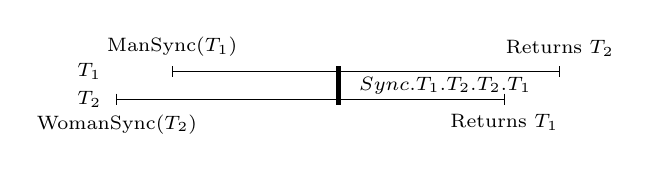
\begin{tikzpicture}[]
  %draw horizontal line
  \draw (2em,0em) -- (16em,0em);
  \draw (2em,2pt) -- (2em,-2pt);
  \draw (16em,2pt) -- (16em,-2pt);
  \draw (1em,0em) node[] { \scriptsize $T_2$};
  \draw (2em,0em) node[below=2pt] { \scriptsize WomanSync($T_2$)};
  \draw (16em,0em) node[below=2pt] { \scriptsize Returns $T_1$};
  
  
  \draw (4em,1em) -- (18em,1em);
  \draw (4em,1em+2pt) -- (4em,1em-2pt);
  \draw (18em,1em+2pt) -- (18em,1em-2pt);
  \draw (1em,1em) node[] { \scriptsize $T_1$};
  \draw (4em,1em) node[above=2pt] { \scriptsize ManSync($T_1$)};
  \draw (18em,1em) node[above=2pt] { \scriptsize Returns $T_2$};
  
  \draw [line width=2pt] (10em,0em-2pt) -- (10em,1em+2pt);
  \draw (10em,0.5em) node[right=4pt] { \scriptsize $Sync.T_1.T_2.T_2.T_1$};
  \end{tikzpicture}
  %}
  \label{menwomen.timeline}
  \caption{Time Line}
\end{figure}

A generic and scalable testing system is introduced to make the test cover as many cases as possible. The testing system includes an arbitrary number of processes, and each process calls any functions provided by the synchronization objects for any finite or infinite number of times. For the CSP implementation, each process non deterministically chooses a function and its parameters, or the process chooses to terminate. Figure \ref{menwomen.csp.testsystem} is the definition of a testing process and a testing system for MenWomen object in CSP.

\begin{cspinline}{menwomen.csp.testsystem}{CSP implementation of the testing processes and system}
Thread(me)=
    (manSync(me);Thread(me))
 |~|(womanSync(me);Thread(me))
 |~|STOP
System(All)=runWith(True,True,||| me:All @ Thread(me))
\end{cspinline}
  
There are two properties one should check for the system. First, the traces of the system are valid. If a thread $t_1$ calls \CSPM{ManSync} and returns the thread identity $t_2$, then $t_2$ must call \CSPM{WomanSync} somewhere. This is done by checking that the system refines a linearization specification (introduced earlier?). Second, the system should not deadlock when matching is possible. This can be done by another specification process, which records the set of men processes and women processes to determine if matching is possible. However, it is easier to modify the linearization specification process and check that the system failure refines the specification process.

The implementation of the linearizer specification relies on the synchronization point. The synchronization point of a man process and a woman process is represented by a \CSPM{Sync} event. The $Sync.t_1.a.t_2.b$ represents the synchronization of a man process $t_1$ with parameter $a$ with a woman process $t_2$ with parameter $b$.

With the \CSPM{Sync} event, it is simple to define the linearizer for a process. The process can choose to call \CSPM{ManSync}, synchronize with a woman process, and return the identity of the woman process. Or, the process can choose to call \CSPM{WomanSync}, synchronize with a man process, and return the identity of man process. Also, the process chooses to terminate when it finishes calling a function.
\begin{cspinline}{menwomen.csp.testsystem}{CSP implementation of the testing processes and system}
Lin(All,me)= (
  Call!me!ManSync->
  Sync!me?mereturn?other?otherreturn ->
  Return!me!ManSync!mereturn ->
  Lin(All,me)
)|~|(
  Call!me!WomanSync ->
  Sync?other?otherreturn!me?mereturn ->
  Return!me!WomanSync!mereturn ->
  Lin(All,me)
)|~|STOP
\end{cspinline}

\section{ABC}
In the ABC object, three threads are involved in each round of synchronization. For simplicity, a process calling \CSPM{syncA}, \CSPM{syncB}, and \CSPM{syncC} is called a A process, B process, C process. In each round of synchronization, A A-process, B-process, and C-process synchronize, and each process returns the argument of two other processes. 

\begin{scalafloat}{abc.scala.correct}{Scala implementation of the ABC using semaphores}
class ABC[A,B,C] extends ABCT[A,B,C]{
  // The identities of the current (or previous) threads.
  private var a: A = _
  private var b: B = _
  private var c: C = _

  // Semaphores to signal that threads can write their identities.
  private val aClear = MutexSemaphore()
  private val bClear, cClear = SignallingSemaphore()

  // Semaphores to signal that threads can collect their results. 
  private val aSignal, bSignal, cSignal = SignallingSemaphore()

  def syncA(me: A) = {
    aClear.down         // (A1)
    a = me; bClear.up   // signal to b at (B1)
    aSignal.down        // (A2)
    val result = (b,c)
    bSignal.up          // signal to b at (B2)
    result
  }

  def syncB(me: B) = {
    bClear.down         // (B1)
    b = me; cClear.up   // signal to C at (C1)
    bSignal.down        // (B2)
    val result = (a,c)
    cSignal.up          // signal to c at (C2)
    result
  }

  def syncC(me: C) = {
    cClear.down         // (C1)
    c = me; aSignal.up  // signal to A at (A2)
    cSignal.down        // (C2)
    val result = (a,b)
    aClear.up           // signal to an A on the next round at (A1)
    result
  }
}      
\end{scalafloat}

For the above semaphore implementation of ABC object, In each round
\begin{itemize}
    \item Initially semaphore \CSPM{aClear} is raised.
    \item An A-process acquire semaphore \CSPM{aClear}, sets the shared variable \CSPM{a} to its parameter, raises semaphore \CSPM{bClear} and waits to acquire semaphore \CSPM{aSignal}. A B-process and a C-process operates in turn with a slight change of semaphore and variable name.
    \item The A-process is able to continue after a C-process raises semaphore \CSPM{aSignal}. The A-process reads the shared variable \CSPM{b} and \CSPM{c}, raises the semaphore \CSPM{bSignal}, and returns. This also happens in turn for the B-process and the C-process.
\end{itemize}

Using the shared variable and semaphore module, it is easy to translate the Scala implementation to a CSP implementation.

Unlike monitor in Java and Scala, raising a semaphore immediately allows another thread waiting to acquire the semaphore to continue. So in the semaphore implementation, it is essential to take a copy of the two other arguments before raising the semaphore.

On the other hand, what if the implementation of \CSPM{syncA} does not take a copy of the argument? It turns out the ABC object still works correctly when only three threads are involved, but fails the linearization test with four threads.

\subsection{Testing}
For the MenWomen object, 
Using the standard linearization testing technique, the following \CSPM{Sync} channel can be used to represent the synchronization of three involved threads. For example, the event $Sync.t_1.a.b.c.t_2.d.e.f.t_3.g.h.i$ represents the synchronizations of three threads, $t_1,t_2,t_3$, in which the first process $t_1$ calls \CSPM{aSync} with $a$ and returns $(b,c)$, the second process $t_2$ calls \CSPM{bSync} with $d$ and returns $(e,f)$, and last process $t_3$ calls \CSPM{cSync} with $g$ and returns $(h,i)$. The spec process should then check that for each synchronization point, the return value of each functional call is the pair of arguments of the two other function call.

\begin{cspinline}{}{}
channel Sync: TypeThreadID.TypeData.TypeData.TypeData.
              TypeThreadID.TypeData.TypeData.TypeData.
              TypeThreadID.TypeData.TypeData.TypeData

Spec = Sync?aid?a?b?c
           ?bid:diff(TypeThreadID,{aid})!b!a!c
           ?cid:diff(TypeThreadID,{aid,bid})!c!a!b 
    -> Spec
\end{cspinline}
//Preparation of test case: I will describe 
There are two test cases. The first test case involves three threads. Each of the thread chooses a data non-deterministically and then calls one of \CSPM{aSync}, \CSPM{bSync}, \CSPM{cSync}. The second test case involves four thread, which chooses a data non-deterministically and calls \CSPM{aSync}. In both cases, the systems should be traced refined (is it this direction in words) by the specification process. In addition, both systems should never deadlock. Because in both system, there are always threads willing to communicate as \CSPM{aSync}, \CSPM{bSync}, \CSPM{cSync} respectively.

When testing with both the correct and the faulty versions of ABC object, FDR finishes the first test case relatively quickly, but requires a long time to finish the second test. With logging message from FDR, it was found the compilation of specification process took the longest time. 
//TODO: Table

\subsubsection{Speeding up model compilation}
Consider the specification process. Let $N$ be the number of threads in the system, $M$ be the size of the set of all possible arguments. The specification process is the alphabetized parallel of $N$ individual linearizers. In each linearizer, the process first chooses to perform one of \CSPM{aSync}, \CSPM{bSync} or \CSPM{cSync}, chooses the argument of the functional call for \CSPM{Call} event, then chooses the rest of arguments for \CSPM{Sync} event, and finally performs one event before recursing into itself.

There are $O(3*N^3M^9)$ different transitions before the individual linearizer recurses into itself. However, according to the specification process, once the argument and return value of \CSPM{syncA} is determined, all remaining arguments and return value are also determined. So only $O(3*N^3M^3)$ transitions are valid according to the specification. 

\begin{cspinline}{}{}
  Call!me!ASync?a->
    Sync!me!a?b?c 
        ?t2:diff(All,{me})?t2b?t2a?t2c 
        ?t3:diff(All,{me,t2})?t3c?t3a?t3b ->
    Return!me!ASync!b!c ->
    Lin(All,me)
\end{cspinline}
    
With the above analysis, it is tempting to optimize the individual linearizer by using the information from the specification process. Instead of choosing all possible remaining arguments, the individual linearizer could choose arguments that are correct according to the specification process.

\begin{cspinline}{}{}
  Sync!me!a?b?c 
      ?t2:diff(All,{me})!b!a!c
      ?t3:diff(All,{me,t2})!c!a!b ->
  Return!me!ASync!b!c
\end{cspinline}

It is possible to further simplify the \CSPM{Sync} channel, as now the arguments representing return value are redundant. This change does not reduce the number of transitions for an individual linearizer, but it may help FDR simulating the model faster.

\begin{cspinline}{}{}
channel Sync: TypeThreadID.TypeThreadID.TypeThreadID.
              TypeData.TypeData.TypeData

Lin(All,me)= (
  Call!me!ASync?a ->
  Sync!me?t2:diff(All,{me})?t3:diff(All,{me,t2})!a?b?c ->
  Return!me!ASync!b!c ->
  Lin(All,me)
) ...
\end{cspinline}

With the above optimizations, the testing finishes quickly for both test cases.

//TOADD: Table of compilation time

\subsubsection{Explanation of the error case}
With the traces of the counterexample from FDR, it is possible to see what goes wrong in the faulty version when there are four threads.

//TODO: Draw diagram using Scala code for this.
\begin{itemize}
  \item Thread $T_A$, $T_B$, $T_C$ call \CSPM{aSync}, \CSPM{bSync} or \CSPM{cSync} respectively, and put down its argument in turn.
  \item Thread $T_A$ raises \CSPM{bSignal} without saving a copy of   return value {(b,c)}. The other two threads $T_B$, $T_C$ are able   to continue and exit. 
  \item Thread $T_D$, $T_B$, $T_C$ call \CSPM{aSync}, \CSPM{bSync} or \CSPM{cSync} respectively, and put down its argument in turn.
  \item Thread $T_A$ uses the wrong overwritten $(b,c)$ as return value. 
  
\end{itemize}

\subsubsection{Conclusion}
In the above section, we tested a semaphore based concurrent datatypes. With the testing result, we showed that it is important to be reminded that a thread waiting for the semaphore to raise can immediately continue and overwrite shared variables, after the semaphore is raised by another process.
\end{document}